\chapter{Security Tools For The Pipeline}

\section{Introduction}
This chapter presents a description of the tools that have been determined for use in this thesis. It will provide a description of each tool and its features, outlining their strengths and weaknesses which was discovered during the testing.  
%\subsection{Astra}
%Astra's pentest suite offers a seamless solution for SMEs to maintain continuous security. It blends automated vulnerability scanning, utilizing over 3000 tests, with manual pentest conducted by security experts. This platform provides authenticated scanning, integration with CI/CD, risk scoring, collaboration features, a resolution center, and verifiable pentest results. Small and medium businesses, lacking a dedicated security team, can benefit from Astra's user-friendly security tools and easily enhance their application's security with minimal technical requirements. Begin by utilizing the automated DAST scanner for an initial security report on your web applications.\cite{astra}
%\subsubsection{Why We Chose Astra}

%\subsection{Mend}
%Mend makes securing developer creations effortless. It eliminates the hassle of application security, enabling development teams to produce secure, high-quality code at a faster pace. As the market leader in securing open source usage in software development, Mend SCA detects, reports, prioritizes, automatically fixes, and prevents open source risks. Mend SAST provides custom code vulnerability detection and prioritization, allowing developers to quickly identify the most pressing software risks in their proprietary code. Additionally, MEND Supply Chain Defender safeguards businesses against supply chain attacks by detecting and blocking harmful open source packages before they can infect your codebase with malicious activity.\cite{mend}
%\subsubsection{Why We Chose Mend}


\section{Snyk}
Snyk is a comprehensive developer security platform that helps secure code, dependencies, containers, and infrastructure as code. It provides thorough scans of the code and alerts the user to any vulnerabilities. Beyond just checking the code, Snyk also examines installed dependencies, Docker containers, infrastructure as code, and more. This platform supports a wide range of programming languages and includes plugins compatible with various \acrlong{ide}s.\cite{snyk}
\subsection{Why We Chose Snyk}

\section{OWASP ZAP}
OWASP Zed Attack Proxy (ZAP) is an open-source web application security scanner. It is free and is maintained by volunteers across the world under the Open Web Application Security Project (OWASP). ZAP is a DAST tool, and is designed to test web application security. ZAP offers functionality for a wide range of people - from developers to experienced testers. ZAP is available in versions that are compatible with major operating systems, as well as Docker, which means that users are not limited to a specific operating system when using the tool.\cite{owaspZAP}


\subsection{Why We Chose OWASP ZAP}


\section{Github Security Tools}

\subsection{Dependabot}
Dependabot is an in-built Github tool that helps developers keep their project dependencies up-to-date. A dependency can be considered a piece of code or software that the project that's being worked on needs and relies on. For example, the project might use a library or package that someone else has written, then this library/package can be considered a dependency of the project. 

Dependencies can be updated over time as new versions are released. Therefore, it is crucial that developers keep the dependencies up to date to ensure that the project stays secure. However, keeping track of all updates that come and manually run these updates can be frustrating for developers since it can be rather time-consuming and error-prone.Dependabot automates the process of checking for new versions of your dependencies and creates pull request to update them, that can be reviewed and merged of the update if necessary. 
Dependabot can also automatically resolve any conflict that may arise when updating dependencies and can even open up separate pull requests for separate dependency updates.  \cite{GithubDependabot2}

Dependabot uses "Github Advisory Database" to check for vulnerable data. This database covers a lot of public vulnerabilities and it uses multiple sources, like \acrlong{cve}, \acrlong{nvd} and more. \cite{GithubDependabot1}

\subsection{Code Scanner}
Github's code scanner uses an in-built tool called codeQL that allows the users to analyze the code that lies in the Github repository to find vulnerabilities and errors in the code. The results of these anlayzes are shown as code scanning alerts in Github.This feature helps identifying existing issues, but also prevents new ones from being introduced. \cite{CodeQL}

CodeQL can be scheduled so that it runs on days that users set. It also makes it possible to trigger the CodeQL to run. Such triggers can be when changes have been done in the repository. 
 Any issues found during the scanning process are displayed as alerts within the repository. This means that developers can divide the different fixes easily between members in the team.  Once a user fixes the code that triggered the alert, it is automatically closed. Additionally, users can monitor the results of code scanning across their repositories or organization using web-hooks and the code scanning API. 
\cite{GithubCodeScanning}




\subsection{Secret Scanner}
Github's Secret scanner is an in-built tool that analyzes the code on all branches to see if there are any secrets within the code. Such secrets can be tokens or private keys. This is the case for archived repositories as well. To authenticate with an external service, developers may require a token or a private key, which can be issued by a service provider. However, if these secrets gets added to the repository, anyone with read access can use these to their advantage and get access to the external service. Therefore it is highly recommended that such secrets are stored outside the repository. However, secret scanning is created to alert on such secrets when detected. Developers can get the
security scanner in two forms: 
\begin{itemize}
    \item \textbf{Secret Scanning alerts for users}
Github's security scanning for users is intended for organizations that have licensed Github Advanced Security and provides the ability to enable and configure scanning for private and internal repositories. This feature allows users to define their own custom pattern-matching rules to identify secrets in code and will report any matches in the security tab of the repository for review by the organization. 

Overall, security scanning for users allows organizations to define their own custom rules and enables scanning for private and internal repositories.

\item \textbf{Secret Scanning alerts for partners}
This feature can be enabled for teams that use the Github Enterprise Cloud and have a license for the Github Advanced Security. This means that, to access this form the repositories has to be owned by an organization that have license to Github Advanced Security. It is not available for repositories that are owned by individuals. 

When Secret Scanning for users is activated, Github will search for secrets used be various of service providers. If any supported secrets are detected, a secret scanning alert will be generated by GitHub Enterprise Cloud.
Github's Secret scanning for partners is intended for  third-party service providers who have partnered with Github to provide pre-defined pattern-matching for identifying secrets in code. This feature is available for all public repositories and will report any matches of these predefined patterns directly to the relevant partner for their review and action. 

Overall, secret scanning for partners focus on providing predefined pattern-matching rules to third-party service providers. 
\cite{GithubSecretScanning}
\end{itemize}

\section{Amazon Web Services Tools}
\subsection{AWS Lambda}
\acrshort{aws} Lambda is considered a serverless compute server and is created for developers to be able to run code in the cloud without having the need to set up any servers. It is an on-demand service, which means that developers only pay for what they use. Lambda can be integrated with many different services in the \acrshort{aws} cloud, which means that developers can build rather complex backends and pipelines. 

\acrshort{aws} Lambda is what is called an "event-driven" service, which means that it executes code as a response to different events created. Such events can be a lot of things, it can for example be events that have been generated from other \acrshort{aws} services like \acrshort{aws} based data processing pipelines or HTTP endpoints. 

Lambda supports a large amount of different programming languages, such as Python, JavaScript and Ruby etc. However, it also allows developers to create custom runtimes for languages that are not necessarily supported. \cite{AWSLamda}



\subsection{AWS CodePipeline}
In short \acrshort{aws} CodePipeline is a "\textit{[...]fully managed continuous delivery service that helps you automate your release pipeline. It allows users to build, test, and deploy code into a test production environment[...]}"
\cite{AWSCodePipeline}

CodePipeline automates the pipeline, which means that the build, test and deploy phases are all automated and CodePipeline runs these when it detects changes in the repository. So when a developer pushes changes to the repository, it detectes this and then starts the process by building these changes and if there are any tests that are configured it runs these. \cite{AWSCodePipeline1}
\begin{figure}[htp]
    \centering
    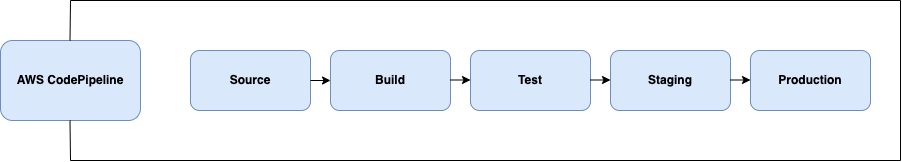
\includegraphics[width=1\columnwidth]{Images/CodePipeline.png}
    \caption{A picture explaining the AWS CodePipeline process}Adapted from: \cite{AWSCodePipeline2}
    \label{fig:my_label}
\end{figure}

\subsection{AWS CodeBuild }
AWS CodeBuild can be described as a "\textit{...fully managed continuous integration service that compiles source code, runs tests, and produces ready-to-deploy software packages.}"
\cite{AWSCodeBuild}
What AWS CodeBuild does is that it downloads the source code provided to it into a build environment and then uses a \Gls{buildspec}.\cite{AWSCodeBuild1}
\begin{figure}[htp]
    \centering
    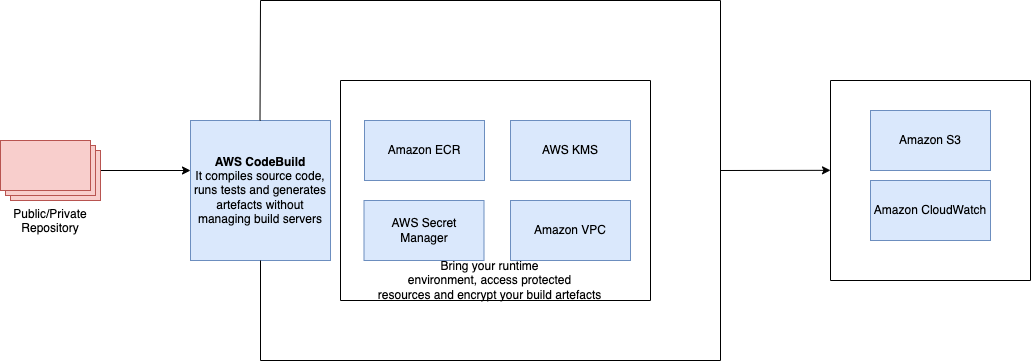
\includegraphics[width=1\columnwidth]{Images/CodeBuild.png}
    \caption{A picture explaining the AWS CodeBuild process}\cite{AWSCodeBuild}
    \label{fig:my_label}
\end{figure}
\newpage
\subsection{AWS CodeCommit}

\acrshort{aws} CodeCommit is defines as "\textit{...a secure, highly scalable, fully managed source control service that hosts private Git repositories.}"
\cite{AWSCodeCommit1}
CodeCommit makes it easier for developers to collaborate on the code and focuses on eliminating the need to operate the source control in the system or scaling the infrastructure. AWS CodeCommit can be necessary for developers who have the need for a secure, reliable and scalable source control system, were code can be stored. \cite{AWSCodeCommit}
\begin{figure}[htp]
    \centering
    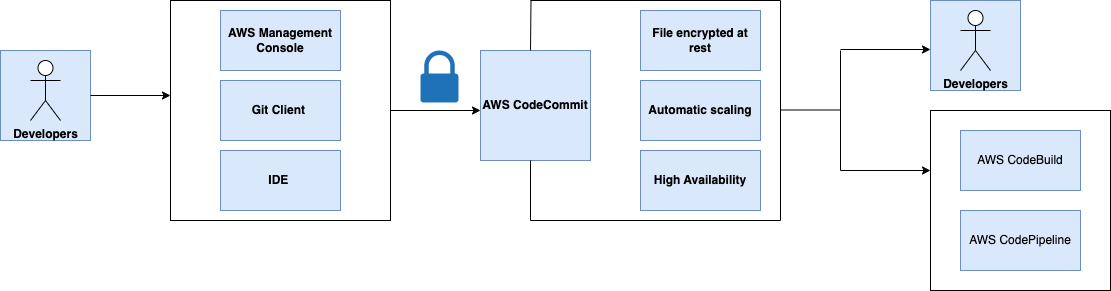
\includegraphics[width=1\columnwidth]{Images/CodeCommit.png}
    \caption{AWS CodeCommit process} Adapted from: \cite{AWSCodeCommit1}
    \label{fig:my_label}
\end{figure}

\newpage
\subsection{AWS CodeDeploy}
\acrshort{aws} CodeDeploy is defined as "\textit{...a fully managed deployment service that automates software deployments to various compute services, such as Amazon Elastic Compute Cloud (EC2), AWS Lamda and more[...]}"\cite{AWSCodeDeploy}.
\acrshort{aws} CodeDeploy helps developers avoid downtime during deployment. It also handles the updating phase of the applications. 

CodeDeploy can deploy code that runs on a server and is store in for example github repositories or in a \acrshort{aws} S3 Bucket. With CodeDeploy, developers does not have to do any changes in the code already existing to use CodeDeploy. \cite{CodeDeploy1}

\begin{figure}[htp]
    \centering
    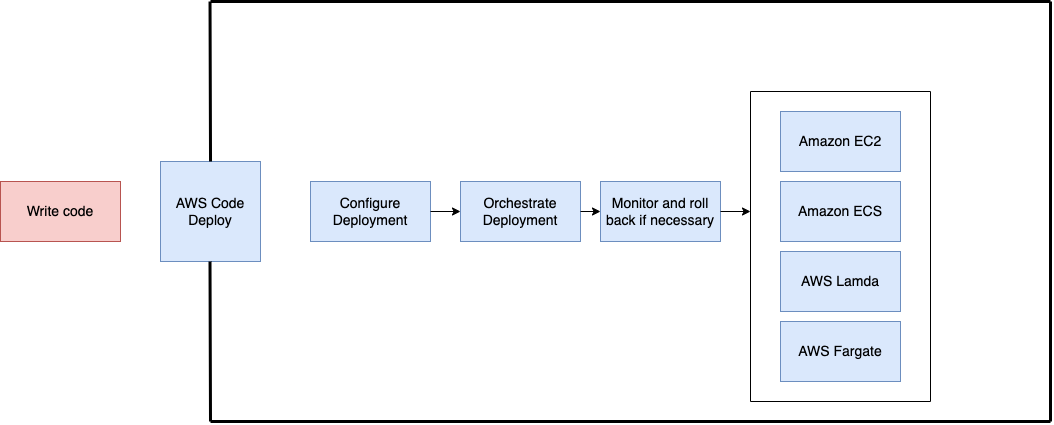
\includegraphics[width=1\columnwidth]{Images/AWSCodeDeploy.png}
    \caption{AWS CodeCommit process} Adapted from: \cite{CodeDeploy1}
    \label{fig:my_label}
\end{figure}

\newpage

\subsection{AWS S3 Bucket}
\acrshort{aws} S3 is a simple storage service which is known to be a cloud-based objective storage service. The S3 bucket is designed to provide users with scalable, durable and highly available storage which can be used to store different types of data. Such data can be documents, photos and so on. 
A S3 bucket can be considered as a container that stores different objects. \cite{S3Bucket}